\documentclass[10pt]{beamer}

\usepackage{polyglossia}
\usepackage{adjustbox}
\usepackage{appendixnumberbeamer}
\usepackage{csquotes}
\usepackage{datetime}
\usepackage{fontspec}
\usepackage{microtype}
\usepackage{color}
\usepackage{url}
\usepackage{hyperref}
\usepackage{amsfonts}
\usepackage{amsmath}
\usepackage{amsthm}
\usepackage{subcaption}
%\usepackage[backend=biber,style=iso-authoryear,sortlocale=en_US,autolang=other,bibencoding=UTF8]{biblatex}
%\usepackage{booktabs}
\usepackage{graphics}
\usepackage{pifont}
\usepackage{ulem}
\usepackage{tikz}


\setdefaultlanguage{english}
\setmainfont{TeX Gyre Termes}
\usetheme{Boadilla}
\usecolortheme{crane}
\setbeamertemplate{title page}[default][rounded=true,shadow=false]
\setbeamertemplate{section in toc}[ball unnumbered]
\setbeamertemplate{bibliography item}{}

\hypersetup{%
	pdfencoding=auto,
	unicode=true,
	citecolor=green,
	filecolor=blue,
	linkcolor=red,
	urlcolor=blue
}

\makeatletter
\newcommand*{\currentSection}{\@currentlabelname}
\makeatother

%\newcommand{\mathmat}{\ensuremath{\mathbf}}
\newcommand{\mathvec}{\ensuremath{\mathbf}}
\newcommand{\vdeg}{\mathrm{d}} % degree of node or edge
\newcommand{\edeg}{\delta} % degree of node or edge

\title[RL for structured data]
{%
	Representation learning for structured data
}

\newdate{presentation}{25}{10}{2025}
\date[October 2025]{ECAI 2025 DC, \displaydate{presentation}}

\author[Marek Dědič]
{%
	Marek~Dědič\inst{1, 2}
}

\institute[CTU in Prague, Cisco]
{%
	\inst{1} Czech Technical University in Prague \and
	\inst{2} Cisco Systems, Inc.
}

\begin{document}

\begin{frame}
	\titlepage
\end{frame}

\begin{frame}{Performance-complexity trade-off in graph representation learning}
	Replace graph \( G \) with a sequence of coarsened graphs \( G_0, G_1, \dots, G_L \). Train model \( M \) on each graph and measure performance and complexity. Stop when the desired trade-off is achieved. \\
	{%
		\raggedleft
		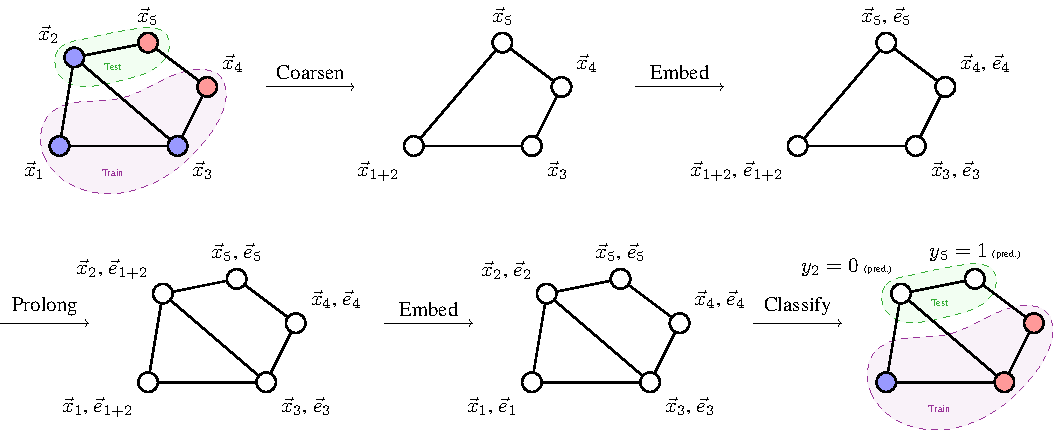
\includegraphics[width=0.5\linewidth]{images/harp-overview/harp-overview.pdf} \\
	}
	\vspace{-140pt}
	{%
		\raggedright
		\vspace{100pt}
		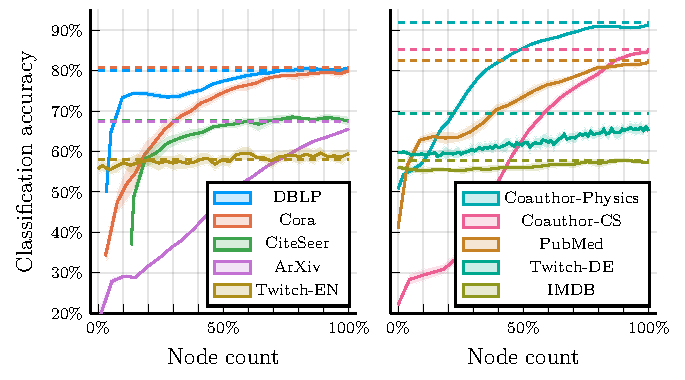
\includegraphics[width=0.5\linewidth]{images/adaptive-coarsening/adaptive-coarsening.pdf}
	}
	\hspace{40pt}
	\raisebox{-20pt}{%
		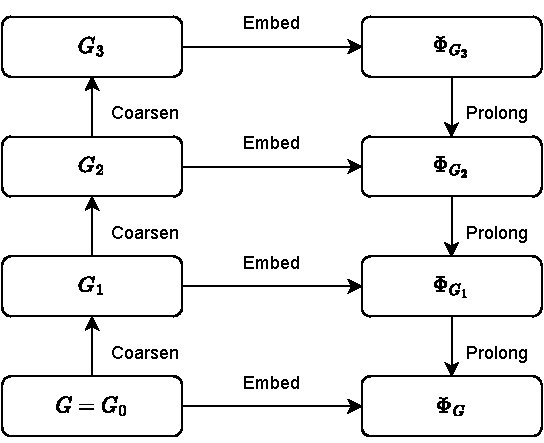
\includegraphics[width=0.25\linewidth]{images/deep-harp/deep-harp.pdf}
	}
\end{frame}

\begin{frame}{Hyperparameter optimization for GNNs}
	\begin{itemize}
		\item Measure graph properties
		\item Train GNN with different hyper-parameters
		\item Train a meta-model predicting GNN performance from graph properties and hyper-parameters
		\item Use the meta-model to suggest hyper-parameters for new graphs
	\end{itemize}

	\begin{center}
		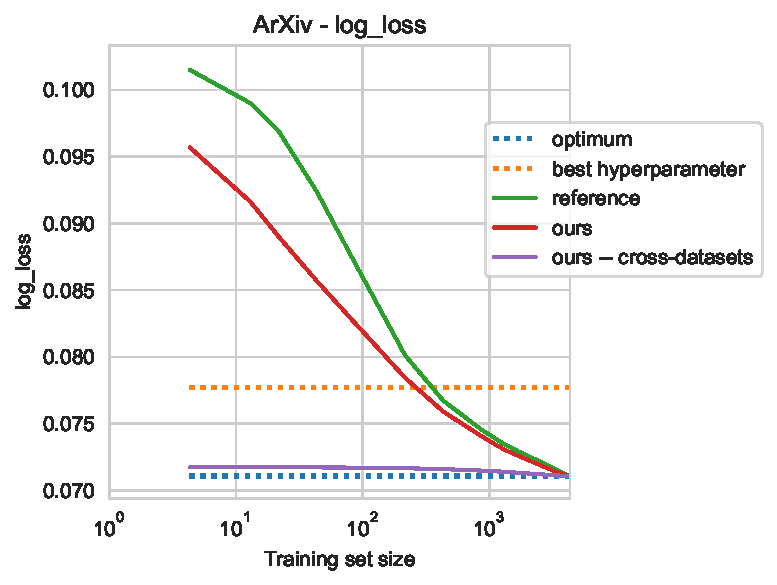
\includegraphics[width=0.6\linewidth]{images/hyperpar_tuning_single.pdf}
	\end{center}
\end{frame}

\end{document}
